\documentclass[a4paper,12pt]{scrartcl}
\usepackage[utf8]{inputenc}
\usepackage[UKenglish]{isodate}
\usepackage{csquotes}
\usepackage{graphicx}
\usepackage{wrapfig}
\usepackage{enumitem}
\usepackage{pdflscape}
\usepackage[toc,page]{appendix}
\usepackage{geometry}
\usepackage{hyperref}
\usepackage{cleveref}
\usepackage{listings}
\usepackage{csvsimple}
\usepackage{booktabs}
\usepackage{longtable}
\usepackage{caption}
\usepackage{subcaption}
\usepackage[colorinlistoftodos]{todonotes}
\usepackage[british]{babel}
\usepackage{float}
%\usepackage[margin=1in]{geometry}
\usepackage{listings}
\usepackage{color}
 
\definecolor{codegreen}{rgb}{0,0.6,0}
\definecolor{codegray}{rgb}{0.5,0.5,0.5}
\definecolor{codepurple}{rgb}{0.58,0,0.82}
\definecolor{backcolour}{rgb}{0.95,0.95,0.92}
 
\lstdefinestyle{mystyle}{
	language=PHP,
    backgroundcolor=\color{backcolour},   
    commentstyle=\color{codegray},
    keywordstyle=\color{magenta},
    numberstyle=\tiny\color{codegray},
    stringstyle=\color{codegreen},
    basicstyle=\footnotesize,
    breakatwhitespace=false,         
    breaklines=true,                 
    captionpos=b,                    
    keepspaces=true,                 
    numbers=left,                    
    numbersep=5pt,                  
    showspaces=false,                
    showstringspaces=false,
    showtabs=false,                  
    tabsize=3,
    morekeywords={ new, __halt_compiler, abstract, and, array, as, break, callable, case, catch, class, clone, const, continue, declare, default, die, do, echo, else, elseif, empty, enddeclare, endfor, endforeach, endif, endswitch, endwhile, eval, exit, extends, final, for, foreach, function, global, goto, if, implements, include, include_once, instanceof, insteadof, interface, isset, list, namespace, new, or, print, private, protected, public, require, require_once, return, static, switch, throw, trait, try, unset, use, var, while, xor}
}

\lstset{language=Java,
  showspaces=false,
  showtabs=false,
  breaklines=true,
  showstringspaces=false,
  breakatwhitespace=true,
  commentstyle=\color{pgreen},
  keywordstyle=\color{pblue},
  stringstyle=\color{pred},
  basicstyle=\ttfamily,
  moredelim=[il][\textcolor{pgrey}]{$$},
  moredelim=[is][\textcolor{pgrey}]{\%\%}{\%\%}
}
 
\lstset{style=mystyle}

\graphicspath{ {images/} }
\usepackage[
	backend=biber,
	style=ieee,
	]{biblatex}

\addbibresource{references.bib}

\title{Programming Project Assignment 1}
\author{Candidate No: 105936}
\date{\today}

\begin{document}
	
	\begin{titlepage}
		\maketitle
	\end{titlepage}
	
	\tableofcontents
	\newpage
	\section{Introduction}
	{
		\begin{figure}[h]
			\centering
			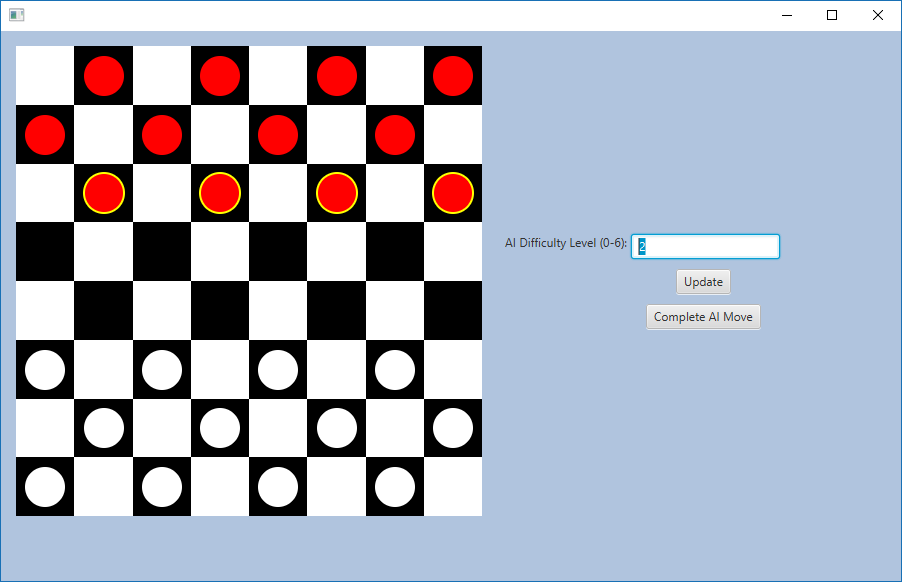
\includegraphics[width=\textwidth]{checkersMain}
			\caption{An Image of the Starting screen for the game}
			\label{img:checkersMain}
		\end{figure}
		\Cref{img:checkersMain} shows the main screen of the game. To start with the user(you) is red and the AI is white these may be referred to dark and light in the document respectively. I probably started developing this the wrong way round developing the GUI and the game part first then adding the AI implemented with minimax later. However the alternative would to make a console game then covert it into a GUI game which probably would have produced a better output but would have taken longer to implement. I originally planed on creating a MVVM GUI application however due to time constraints and difficulty setting up the mvvm project in JavaFX with mvvmFX I decided to not follow a formal framework/structure as it would have taken more time to learn and implement. I have a number of classes in my project:
		\subsection{Main}{My main class focuses on the visuals as all of the GUI code is in this class and it also manages some of the control as well as this allows the user to interact with the board.}
		\subsection{AI}{This class contains the minimax function and the evaluation function more time could and probably should have been spend on the evaluation function. I will go on in more detail about how the evaluation function works further on in the document.}
		\subsection{Colour}{This is actually a very simple enum which is used to identify the two different players Light and Dark}
		\subsection{Draught}{This represents a draught piece and contains it's location information if it is crowned and its Colour.}
		\subsection{Game}{This manages the game and the game board state if I were redoing the project from scratch I probably would have separated out the game board data from the methods and logic as this lead to problems when implementing minimax. The game class contains methods for:
			\begin{itemize}
				\item {finding possible moves}
				\item {carrying out moves}
				\item {the successor function}
				\item {checking for a winner}
			\end{itemize}	
			This contains the majority of the logic for the game internals.
		}
		\subsection{Move}{This represents the movement of a draught and allows me to separate out some logic. And allows me to store a turn choice as an object which can be passed to other classes.}
		\subsection{Capturing Move}{This class extends the move class and allows me to store capturing moves as a different but compatible type. This is mainly because if you capture a draught and it is possible to capture another you get to continue your turn therefore it is vital to store the difference.}		
	}

	\section{Program Functionality}{
		\subsection{Game Internals}
		{
			\subsubsection{Interactive Checkers Gameplay}{
				As mentioned in the introduction I started by developing the game internals and the GUI therefore the gameplay is fairly smooth and functionally correct in terms of rules of the game. The way it works is the Main class asks for a list of possible moves from the game object and then displays them to the user for them to then decide what move to make once chosen it is run through the select move function in the game class which carries out the move for the player. For the AI a similar thing happens once the user presses the complete AI move button then the Main class gets the game and passes it to the AI which returns a move which the Main thread then passes on to the game object. 
				The user starts as the red/dark player and the AI is the white/light player.
			}
			\subsubsection{Valid State Representation}{
				The state representation used is the Game class which can be found at \cref{appedix:Game} and its made up of the following
				\paragraph{Draughts Array List}
				{
					An array list holds the draughts which are on the board currently. the draughts are stored in random order and their position information is stored in the draught class itself. The draughts also store colour information. The position information is an x and y coordinate starting from the top left of the board as that makes it easy to display in the GUI. 
				}
				\paragraph{Current Turn}
				{
					This stores the colour of the current player so the game object knows who's turn it is and therefore which moves to return when calculating them.
				}
				
				\paragraph{Selected Draught}
				{
					This is used for the completing of multiple jumps in one turn as if the player has the option to perform multiple jumps it is only possible to make moves on the draught which completed the original jump and then only if a jump is available.
				}
				\paragraph{Multi-step move}
				{
					This stores if the game is currently a part of a multi step move this means that the game can restrict the moves to only the currently selected draught.
				}
				\paragraph{Game Winner}
				{
					This stores which colour is the game winner so that Main class can display to the user which colour is the winner when the game completes. 
				}
				\paragraph{Game Complete}
				{
					This stores if the game is complete or not. and therefore display who the winner is to the user from the main class.
				}
			}
			\subsubsection{Successor function}{
				The calculation of the moves is in three steps firstly the draught calculates its possible moves given its position and if its crowned or not and removes any which aren't in bounds.
				Secondly the Game class then removes any blocked moves unless it can make a jump.
				Thirdly the \lstinline|findAllPossibleMoves()| method checks for if we are currently in a multi-step move and if so restricts the moves accordingly otherwise it gets all of the moves for the current players draughts.
				It also makes use of the \lstinline|findAllPossibleMoves()| method which works by firstly checking if we are currently on a multi-step move and if so only returning the valid capture moves from the selected draught.
				The function that I have named successor is the function in the Game class \cref{appedix:Game} which returns a following game object when passed a move.
			}
			\subsubsection{Use of Successor Function}{
				The find all moves method is used in both the game and AI classes and the find moves method is used in the main class to display the possible moves for each draught. The find all moves is used in the game class to check if there are possible moves if there aren't then the other player wins.
				It is used in the AI class as a part of the minimax method to get the children of the current game board state. The successor functions don't specifically validate the moves however the only moves either the AI or user have available to them come from the successor function therefore they must be valid.
			}
			\subsubsection{Invalid User Moves}{Invalid user moves are handled by simply not providing the function to complete incorrect moves or more accurately only providing the options to select valid moves. As there is no way for a user to select an incorrect move there is no explanation given with one exception. If the user attempts to deselect the draught during a multi-step move the program gives an error warning with an explanation saying they are only able to move the currently selected draught.
			}
			\subsubsection{Minimax Evaluation}{
				The minimax algorithm has been implemented in the AI class \cref{appendix:AI}.
			}
			\subsubsection{Variable AI difficulty}{}
			\subsubsection{Valid AI Moves}{}
			\subsubsection{Multi-step User Moves}{}
			\subsubsection{Multi-step AI moves}{}
			\subsubsection{Forced Takes}{}
			\subsubsection{Automatic King Conversion}{}
		}
		\subsection{HCI/GUI}
		{
			\subsubsection{Board Representation on Screen}{}
			\subsubsection{GUI Updates}{}
			\subsubsection{Full Graphical Board Display}{}
			\subsubsection{Interactive GUI}{}
			\subsubsection{Mouse Interaction}{}
			\subsubsection{GUI pauses on multi-step moves}{}
			\subsubsection{Display of basic game rules}{}
			\subsubsection{Possible moves display}{}
		}
		
	}
	
	
	\newpage
	\begin{appendices}
	\label{Appendix:start}
	\section{Lab Exercise 1}
	{
		\subsection{Part 1}
		{
			\label{appendix:ex1-1}
			\lstinputlisting[language=c++]{CodeListings/Ex1/mainPart1.cpp}
		}
		\subsection{Part 2}
		{
			\label{appendix:ex1-2}
			\lstinputlisting[language=c++]{CodeListings/Ex1/mainPart2.cpp}
		}
		\subsection{Part 3}
		{
			\label{appendix:ex1-3}
			\lstinputlisting[language=c++]{CodeListings/Ex1/mainPart3.cpp}
		}
	}
	\section{Lab Exercise 2}
	{
		\label{appendix:ex2}
		\subsection{Part 1 - Master Program}
		{
			\label{appendix:ex2-1}
			\lstinputlisting[language=c++]{CodeListings/Ex2/main-master.cpp}
		}
		\subsection{Part 2 - Slave Program}
		{
			\label{appendix:ex2-2}
			\lstinputlisting[language=c++]{CodeListings/Ex2/main-slave.cpp}
		}
	}

\end{appendices}
	\printbibliography[heading=bibintoc,title=References]
\end{document}
